\documentclass[conference,10pt]{IEEEtran}
\IEEEoverridecommandlockouts
\usepackage[T1]{fontenc}
\usepackage{graphicx,booktabs,amsmath,amssymb,multirow,xcolor,url,xspace}
\usepackage[hidelinks]{hyperref}
\hypersetup{pdftitle={Egocentric Human Demonstrations for a Bimanual Robot, Part I: Three-Cube Stacking}, pdfauthor={Jeong Hwan Lee}}
\newcommand{\mm}{\,mm\xspace}

\begin{document}
\title{Egocentric Human Demonstrations for a Bimanual Robot\\Part I: Three-Cube Stacking}
\author{\IEEEauthorblockN{Jeong Hwan Lee}
\IEEEauthorblockA{Technical report, version 4, 7 October 2026 \quad alnrg2arg@gmail.com\\
Short version; Part II covers single-arm approach data. Code, results and sample data are available on request.}}
\maketitle

\begin{abstract}
We study how far egocentric demonstrations recorded with a hand-worn UMI-style gripper can be turned into training data for a
bimanual robot policy. We collected 349 demonstrations of three-cube stacking in six balanced orders and processed them in two
generations. First, MASt3R-SLAM wrist poses with per-episode IMU scale were retargeted to robot joints; a 0.9B X-VLA model trained
on the 561 surviving segments predicts the direction of held-out moving human motion (cosine 0.90 at 1.2\,s, 39.9\mm error) but
predicts spurious motion in static phases and makes no task-useful use of the order instruction. Second, whole episodes were
converted to the robot's own relative Cartesian action contract with no feasibility filter (330 episodes, 48{,}411 training
rows). With a shared contract the remaining human-to-robot gap is visual: an ego-only model gives no useful action direction on
robot frames, and swapping inputs locates the gap in the wrist images. As an initialization, ego pretraining speeds up early robot
fine-tuning, on 312 and on 30 robot episodes alike, but the training-loss advantage disappears (by 60k steps on 312 episodes; by
about 100k--200k steps on 30). An ego-initialized model fine-tuned on 312 robot episodes stacked three cubes in closed loop, but
trials were not counted, so we report a demonstration, not a success rate.
\end{abstract}

\section{Introduction}
Egocentric human demonstrations are cheaper to collect than robot teleoperation, and hand-worn grippers such as
UMI~\cite{chi2024umi} make the human end-effector look like the robot's. Whether such data transfer to a specific robot depends on
calibration, metric pose recovery, conversion into the robot's action space and filtering, each of which can silently change what
a policy learns. EgoMimic~\cite{kareer2024egomimic} and MimicPlay~\cite{wang2023mimicplay} report closed-loop gains from human
video; we instead audit one complete pass through this chain on real data. The question is narrow: \emph{after all processing,
how much robot-executable action structure does a pretrained vision-language-action (VLA) model learn from egocentric human
demonstrations, and does it help robot fine-tuning?} Evaluation is mostly offline or training-loss based; layouts were not
recorded and all six orders appear in training, so we test neither spatial nor task-order generalization. This short version
condenses the full report (kept in the repository) and brings run status to 7 October 2026.

\section{Data and Poses}\label{sec:data}
\textbf{Device and task.} Each hand wears a HandUMI unit: a 1080p30 fisheye wrist camera, a 200\,Hz IMU and a jaw encoder; a
fixed Logitech C922 records the table. Three 50\mm cubes are stacked on a plate in one of six orders named by the instruction.
One operator recorded 349 episodes in 15 sessions on 15--17 September 2026 (2.20\,h; median 23.05\,s), with the next order chosen
as the least collected (51--64 per order), so orders are balanced, not randomized. Cube layouts varied through manual resets but
were not recorded (Fig.~\ref{fig:dataset}). A later robot-like session (HRL80) added 60 episodes, 10 per order.

\begin{figure*}[t]
\centering
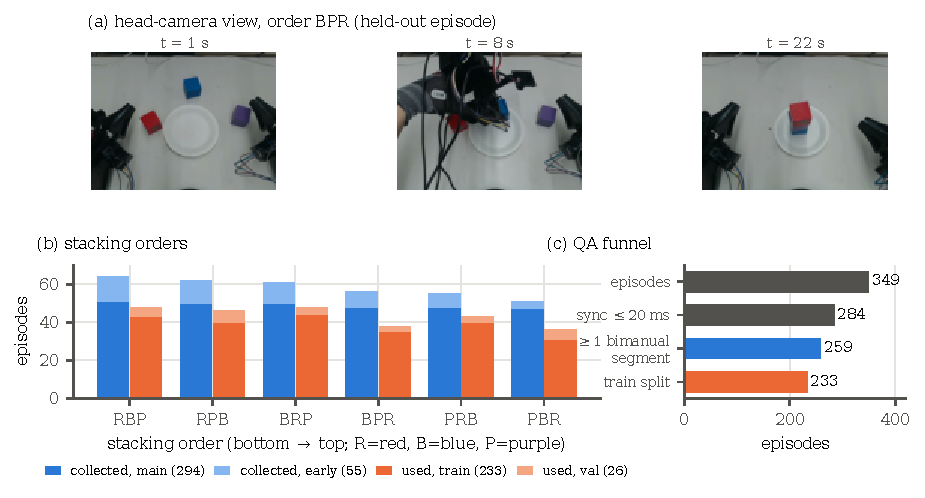
\includegraphics[width=\textwidth]{figures/fig2_dataset.pdf}
\caption{Dataset design. (a) Head-camera frames at 1, 8 and 22\,s of a held-out episode (order BPR). (b) Episodes per stacking
order, as collected and after generation-1 processing. (c) Episode-level funnel.}
\label{fig:dataset}
\end{figure*}

\textbf{Calibration.} Kannala--Brandt fisheye intrinsics; Kalibr~\cite{furgale2013kalibr} camera--IMU calibration with time offsets
of 30.2 and 32.8\,ms and mean reprojection errors of 6.0 and 5.6\,px, high enough that pose accuracy is validated separately; a
caliper camera-to-TCP transform measured on one unit.

\textbf{Wrist poses.} UMI's per-scene ORB-SLAM3 map failed on our data (median coverage 0.03, frequent reversals). We run
MASt3R-SLAM~\cite{murai2025mast3rslam} on the RGB video alone and recover metric scale per episode from the IMU. On 14 ArUco
benchmark episodes this gives coverage 1.00 versus 0.03, scale error p50/p90 4.6/17.0\% (18.5/23.8\% for one global constant),
rotation error p50 0.84\textdegree{} and a 16-step relative position error p90 of 11.3\mm.

\section{Generation 1: Joint-Space Retargeting}\label{sec:gen1}
\textbf{Processing.} Each TCP trajectory is retargeted by IK to the reBot B601 6-DoF arm, re-anchored at a fixed robot start pose.
65 episodes fail the $\le$20\,ms synchronisation requirement; of 1{,}306 candidate bimanual 65-frame segments, 677 leave the robot
workspace, 50 fail the metric check and 18 fail IK, leaving 561 (43.0\%) from 259 episodes, split by episode into 233 train / 26
val. We fine-tune X-VLA~\cite{zheng2025xvla} (879M parameters, from \texttt{xvla-base}, via LeRobot~\cite{cadene2024lerobot}) to
predict 30-step chunks of joint displacements from three views, the instruction and a 14-D state, for 300k steps.

\begin{table}[t]
\centering\footnotesize\setlength{\tabcolsep}{5pt}
\caption{Offline held-out results, final 300k checkpoint (26 episodes). TCP error: median FK position error (mm); MAE: joint
MAE (deg), zero-motion predictor in parentheses.}
\label{tab:results}
\begin{tabular}{@{}llccc@{}}
\toprule
Subset & Metric & $k{=}1$ & $k{=}8$ & $k{=}30$ \\
\midrule
All (798) & TCP err. & 1.5 & 2.2 & 5.7 \\
 & MAE & 0.30 (0.15) & 0.42 (0.25) & 0.97 (0.51) \\
\midrule
Moving (187) & TCP err. & 11.2 & 19.4 & 39.9 \\
 & MAE & 2.02 (2.32) & 3.29 (4.38) & 6.59 (8.68) \\
 & cosine & 0.72 & 0.84 & 0.90 \\
\bottomrule
\end{tabular}
\end{table}

\textbf{Offline results} (Table~\ref{tab:results}, Fig.~\ref{fig:eval}). Errors over all samples are small (1.5--5.7\mm) because
77\% of samples are near-static. On the 23.4\% that move at least 20\mm, the error at $k{=}30$ (1.2\,s) is 39.9\mm, the direction
cosine rises from 0.72 to 0.90, and joint MAE is 13--32\% below a zero-motion predictor (6.59 versus 8.68\textdegree{} at $k{=}30$).
On all samples the policy is \emph{worse} than predicting no motion: it creeps during static phases. \textbf{Prompt swap.} The six
order instructions move the prediction by 4.8\mm at $k{=}30$ (50$\times$ the noise spread, but 8\% of the 62\mm predicted
displacement), and the true instruction's mean rank is 3.55 of 6 (chance 3.5): the model makes no task-useful use of the order.

\begin{figure*}[t]
\centering
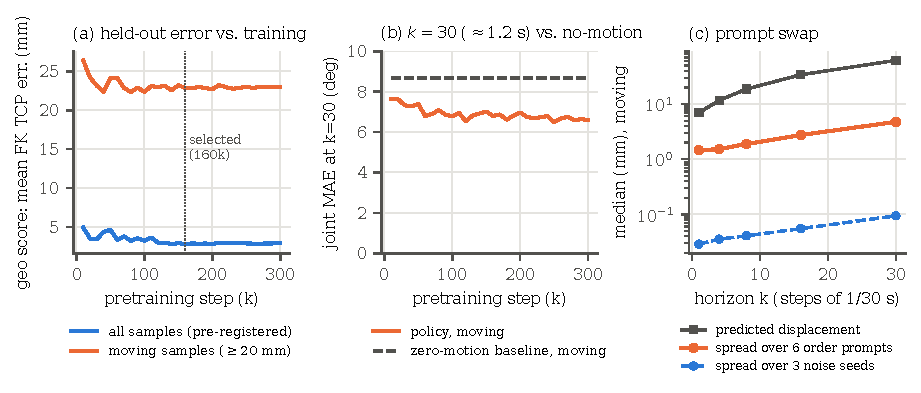
\includegraphics[width=0.92\textwidth]{figures/fig4_eval.pdf}
\caption{Generation-1 offline evaluation. (a) Geo score over training, all versus moving samples. (b) Joint MAE at $k{=}30$ on
moving samples, policy versus zero-motion predictor. (c) Prompt swap: spread across six instructions versus three noise seeds.}
\label{fig:eval}
\end{figure*}

\textbf{Retargeting v2 and fine-tuning.} The single start anchor was the main loss. Retrieving the closest feasible robot
trajectory window (calibrated on 30 robot episodes, measured on 120 others) raises usable segments from 36.5\% to 56.1\% (Table~\ref{tab:retarget}) and
brings postures close to real robot postures (nearest-neighbour distance 1.49$\to$0.27\,rad, start clusters 1$\to$100). The
robot-like re-collection halved live wrist-rotation speed but raised usable segments only to 58.9\%: workspace placement, not
style, is the limit. Fine-tuned on 150 robot episodes, the ego-initialized model has a 10\% lower geo score than one trained from
the base model (95\% CI 5.6--14.7\%), but only on episodes inside both training sets, so this measures fit, not generalization.

\begin{table}[t]
\centering\footnotesize\setlength{\tabcolsep}{3.5pt}
\caption{Retargeting variants on 1{,}229 candidate segments, measured against 120 held-out robot episodes. NN: nearest-neighbour
joint distance to robot postures (rad, p50/p90).}
\label{tab:retarget}
\begin{tabular}{@{}lccc@{}}
\toprule
Variant & Usable & NN p50 / p90 & Start clusters \\
\midrule
v1 single anchor & 36.5\% & 1.49 / 1.55 & 1 \\
v2-K multi-seed IK & 66.6\% & 1.21 / 1.60 & -- \\
v2-Kr + posture penalty & 67.0\% & 0.44 / 0.74 & -- \\
v2-TR window retrieval & 56.1\% & 0.27 / 0.45 & 100 \\
\bottomrule
\end{tabular}
\end{table}

\section{Generation 2: Cartesian Ego Data}\label{sec:gen2}
\textbf{Contract.} Joint retargeting removed a third to a half of the motion and used a different action space from our robot
policies. Generation 2 converts each wrist trajectory directly into the robot data's representation: rows at 15\,Hz; an action
chunk of 16 relative poses $T(t)^{-1}T(t+k\Delta)$, $\Delta=50.05$\,ms (0.8\,s), interpolated on the raw 30\,Hz track; per arm
position, 6-D rotation and gripper (20 dimensions, ``CART20''), the rest of the 32-D head zeroed; state relative to each arm's
task start. Source: 273 original and 60 HRL80 episodes, 330 after IMU-scale checks, with no workspace or IK filter.

\textbf{Silent pose jumps.} Ego states showed jumps above 100\mm that the robot data lacks. 1{,}482 of the 2{,}598 apparent jumps
above 30\mm were time gaps between non-adjacent rows; the rest were real one-frame MASt3R-SLAM jumps without a tracking-loss
flag, which corrupt every later start-anchored state. Truncating an episode after such a jump leaves 297 train episodes and
48{,}411 rows ($-6.20$\%); the largest adjacent-row step falls from 422.5 to 90.5\mm.

\textbf{Ego versus robot.} The robot's IK reaches 99.7\% (left) and 99.5\% (right) of ego positions. Ego hands use a smaller
workspace and are both still far more often (19.5\% versus 2.4\% of samples). The largest difference is visual: wrist-image
sharpness (Laplacian variance) has a median of 1{,}854/1{,}487 for ego fisheye views and 59/64 for the robot's wrist cameras.

\section{Transfer to the Robot}\label{sec:transfer}
All runs use one recipe: X-VLA with loss on action dimensions 0--19, batch 8, 8-bit AdamW (policy learning rate $10^{-4}$), bf16,
seed 1000; fine-tuning uses robot normalization statistics. R312c is 312 teleoperated robot episodes of the same task.

\textbf{Which soft prompt?} X-VLA selects soft prompts by an embodiment id. In the public base weights only slots 10--17 were ever
trained; the ids 0 and 6 we had used were untrained. All runs below use the unused slot 20.

\begin{table}[t]
\centering\footnotesize\setlength{\tabcolsep}{3.2pt}
\caption{Ego-only checkpoint (40k), median direction cosine at $k{=}4/8/16$ (left $|$ right) when images and state come from
different domains.}
\label{tab:ablation}
\begin{tabular}{@{}lcc@{}}
\toprule
Images + state & Left $k$=4/8/16 & Right $k$=4/8/16 \\
\midrule
ego + ego & 0.87 / 0.91 / 0.92 & 0.89 / 0.94 / 0.84 \\
ego + robot & 0.76 / 0.81 / 0.90 & 0.72 / 0.69 / 0.72 \\
robot + robot & 0.36 / 0.30 / $-$0.01 & 0.19 / 0.02 / $-$0.15 \\
robot + ego & 0.16 / 0.24 / $-$0.16 & 0.49 / 0.33 / $-$0.03 \\
\bottomrule
\end{tabular}
\end{table}

\textbf{The gap is in the wrist images.} On 120 robot frames, an ego-only model (40k steps) has a median direction cosine at
0.4\,s of $-0.05$/$-0.03$ (left/right), versus $+0.81$/$+0.77$ for a robot-trained reference; no axis or arm swap raises it above
$+0.16$. Swapping inputs between domains (Table~\ref{tab:ablation}), the ego model keeps a cosine of 0.69--0.90 with ego images whatever state it gets (robot
state included), and falls to between $-0.25$ and $+0.49$ with robot images whatever the state. Re-rendering ego wrist frames as
robot-like pinhole views (ROBOT100) lowers their sharpness to 181/132, still 2--3$\times$ the robot's; a 300k pretraining on this
data finished on 5 October (training loss 0.007).

\textbf{Initialization on 312 robot episodes.} Fine-tuned on R312c from the base model (A) and from a 50k ego checkpoint (B) with
identical data, schedule and seed, B starts at a 3.9$\times$ lower loss (0.945 for A and 0.244 for B at step 200); the ratio
B/A is 0.49 over the first 5k steps, 0.875 over 5k--20k and 0.95 over 20k--40k, and the two are tied by 60k (0.0733 versus
0.0745; Fig.~\ref{fig:egoinit}). Training loss only, one seed per arm; there is no held-out or closed-loop comparison of A and B.

\begin{figure*}[t]
\centering
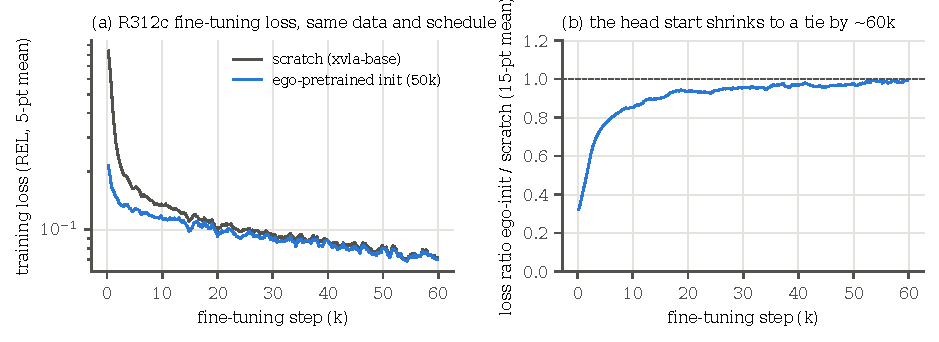
\includegraphics[width=0.72\textwidth]{figures/fig5_ego_init_loss.pdf}
\caption{R312c fine-tuning from the base model versus from the 50k ego checkpoint, same data, schedule and seed. (a) Training
loss. (b) Ratio; values below 1 favour the ego initialization.}
\label{fig:egoinit}
\end{figure*}

\textbf{Initialization on 30 robot episodes.} To test the regime where human data should matter, we fine-tuned on R30 (R312c
episodes 150--179, 17{,}600 frames, 600k-step schedule) from the base model and from the ROBOT100 pretraining at 100k and 300k
steps (Table~\ref{tab:r30}, Fig.~\ref{fig:r30}). Both ego initializations start below half the scratch loss (window ratio 0.544
and 0.493 over 1k--5k); the 100k initialization reaches parity by about 100k steps (0.970 over 50k--100k, 1.021 over 100k--150k),
the 300k one by about 200k. The 100k checkpoint is mid-schedule, and the 300k arm ran on a different GPU and PyTorch version, so
the arms are not exact twins. All three were stopped at 471k, 305k and 310k steps after 139--214 epochs: every arm memorizes 30
episodes. No R30 checkpoint has been run on the robot.

\begin{table}[t]
\centering\footnotesize\setlength{\tabcolsep}{4pt}
\caption{R30 fine-tuning: training loss at matched steps and window-mean ratio to scratch ($<$1 favours ego). One seed per arm.}
\label{tab:r30}
\begin{tabular}{@{}lccc@{}}
\toprule
Step / window & Scratch & Ego-PT 100k init & Ego-PT 300k init \\
\midrule
200 & 0.801 & 0.239 & 0.446 \\
10k & 0.065 & 0.056 & 0.040 \\
100k & 0.009 & 0.009 & 0.007 \\
\midrule
ratio 1k--5k & & 0.544 & 0.493 \\
ratio 50k--100k & & 0.970 & 0.856 \\
ratio 100k--150k & & 1.021 & 0.914 \\
\bottomrule
\end{tabular}
\end{table}

\begin{figure*}[t]
\centering
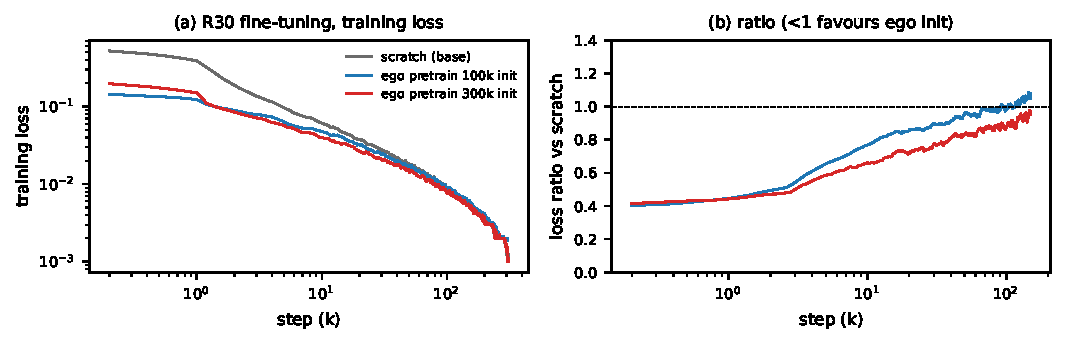
\includegraphics[width=0.72\textwidth]{figures/fig8_r30_ablation.pdf}
\caption{R30 fine-tuning from the base model and from ego pretraining at 100k and 300k steps. (a) Training loss. (b) Ratio to
scratch up to 150k. Training loss only.}
\label{fig:r30}
\end{figure*}

\textbf{On the robot.} Between 2 and 4 October 71 checkpoints ran 49{,}431 control cycles, but the cycle log records IK tracking,
not task outcome. The ego-initialized model fine-tuned on R312c for 300k (B300, checkpoints 75k--205k) completed the full
three-cube stack in closed loop; trials were not counted and no video was taken, so this is a demonstration with no success rate,
and no scratch model on the same data was tested under the same protocol. Only the 150k and 200k B300 checkpoints survive a later
storage clean-up. A trial logger now exists in the deployment interface but has recorded no trial.

\section{Lessons, Limitations and Next Steps}
(i) A pretrained model's conditioning interface must be audited: two of our ids pointed at untrained soft prompts. (ii) With a
shared tensor contract, swapping inputs between domains localizes the gap, here to the wrist images. (iii) Pose and scale sources
fail silently in some regime (one-frame SLAM jumps here, IMU scale on slow motion in Part II); an independent reference catches it.
(iv) Training-loss comparisons of initializations end in a tie once robot data is memorized, at 312 and at 30 episodes alike;
only held-out or closed-loop tests at early checkpoints can show a benefit.

\textbf{Not supported by this study:} a closed-loop success rate; any closed-loop difference between ego-initialized and scratch
models; generalization to new layouts or unseen orders; transfer beyond one operator and one scene; transfer of the ego-only
policy or the re-rendered images to robot cameras. \textbf{Next:} log every robot trial (checkpoint, layout, instruction, stack
level 0--3, wrong colour, failure reason) with 20--30 trials per model; compare the R30 arms closed-loop at early and middle
checkpoints (10k--150k); record layouts and hold out layout regions and two orders.

\begin{thebibliography}{9}\footnotesize
\bibitem{chi2024umi} C.~Chi \emph{et al.}, ``Universal manipulation interface: In-the-wild robot teaching without in-the-wild robots,'' in \emph{RSS}, 2024.
\bibitem{kareer2024egomimic} S.~Kareer \emph{et al.}, ``EgoMimic: Scaling imitation learning via egocentric video,'' \emph{arXiv:2410.24221}, 2024.
\bibitem{wang2023mimicplay} C.~Wang \emph{et al.}, ``MimicPlay: Long-horizon imitation learning by watching human play,'' in \emph{CoRL}, 2023.
\bibitem{furgale2013kalibr} P.~Furgale, J.~Rehder, and R.~Siegwart, ``Unified temporal and spatial calibration for multi-sensor systems,'' in \emph{IROS}, 2013.
\bibitem{murai2025mast3rslam} R.~Murai, E.~Dexheimer, and A.~J. Davison, ``MASt3R-SLAM: Real-time dense SLAM with 3D reconstruction priors,'' in \emph{CVPR}, 2025.
\bibitem{zheng2025xvla} J.~Zheng \emph{et al.}, ``X-VLA: Soft-prompted transformer as scalable cross-embodiment vision-language-action model,'' in \emph{ICLR}, 2026.
\bibitem{cadene2024lerobot} R.~Cadene \emph{et al.}, ``LeRobot: State-of-the-art machine learning for real-world robotics in PyTorch,'' 2024.
\end{thebibliography}
\end{document}
